% ICIIT 2027 submission version (ACM sigconf). Compiler: pdfLaTeX. Bibliography: BibTeX (ACM-Reference-Format).
% Content is shared with ../paper (IEEE version for the course). Edit content in ../paper first, then copy here.
% Tables in tables/*.tex and figures/summary_deltas.pdf are generated by `python -m src.paper_tables`.
\documentclass[sigconf]{acmart}

\usepackage{float}
\usepackage{multirow}
\usepackage{tikz}
\usetikzlibrary{positioning,arrows.meta,fit}
\setlength{\emergencystretch}{2em}

\AtBeginDocument{\providecommand\BibTeX{{Bib\TeX}}}

\setcopyright{none}
\settopmatter{printacmref=false}
\renewcommand\footnotetextcopyrightpermission[1]{}
\acmConference[ICIIT 2027]{2027 12th International Conference on Intelligent Information Technology}{March 04--07, 2027}{Ho Chi Minh City, Vietnam}

\begin{document}

\title[Evaluation Leakage in FR/NFR Requirements Classification]{How Much Does Evaluation Leakage Inflate FR/NFR Requirements Classification? A Leakage-Aware Re-Evaluation of Single and Ensemble Classifiers}

\author{Nguyen Phat Tai}
\email{tainpse184284@fpt.edu.vn}
\affiliation{%
  \institution{FPT University}
  \city{Ho Chi Minh City}
  \country{Vietnam}}

\author{Hoang Anh}
\email{hoanganh.21022005@gmail.com}
\affiliation{%
  \institution{FPT University}
  \city{Ho Chi Minh City}
  \country{Vietnam}}

\renewcommand{\shortauthors}{Nguyen et al.}

\begin{abstract}
Some studies on classifying functional (FR) and non-functional (NFR) requirements report accuracies of 98\% to 99\%. We examined three distinct evaluation concerns: duplicate rows shared across random folds, oversampling before splitting, and generalisation to unseen projects. Only the first two are leakage mechanisms; project-grouped evaluation measures performance on a different deployment setting. We measured their effects on PROMISE\_exp (969 requirements, 47 projects), with a replication on the Dalpiaz et al.\ data. We evaluated seven classifiers, including a dummy baseline, hard voting and stacking, under stratified, duplicate-grouped and project-grouped 5-fold CV repeated with 5 seeds. Model comparisons on the same splits used the corrected repeated $k$-fold $t$-test with Holm adjustment. Differences between protocols are reported descriptively. The protocol was locked before any run. Oversampling before splitting raised macro-F1 on the 12-class task by 0.39 to 0.49, to between 0.95 and 0.99. On the binary task the increase was 0.02 to 0.03. Testing on unseen projects lowered macro-F1 by 0.13 to 0.19 and changed the model ranking. Grouping the few duplicates changed macro-F1 by less than 0.01, and the ensembles beat only the random forest. We recommend oversampling inside the training fold, reporting duplicate handling and project-level results, and testing on the same folds before ranking models.
\end{abstract}

\begin{CCSXML}
<ccs2012>
 <concept>
  <concept_id>10011007.10011074.10011075.10011076</concept_id>
  <concept_desc>Software and its engineering~Requirements analysis</concept_desc>
  <concept_significance>500</concept_significance>
 </concept>
 <concept>
  <concept_id>10010147.10010257.10010258.10010259.10010263</concept_id>
  <concept_desc>Computing methodologies~Supervised learning by classification</concept_desc>
  <concept_significance>300</concept_significance>
 </concept>
</ccs2012>
\end{CCSXML}

\ccsdesc[500]{Software and its engineering~Requirements analysis}
\ccsdesc[300]{Computing methodologies~Supervised learning by classification}

\keywords{requirements classification, functional and non-functional requirements, data leakage, evaluation methodology, oversampling, ensemble learning}

\maketitle

\section{Introduction}
\label{sec:intro}

Separating functional requirements (FR) from non-functional requirements (NFR) early helps analysts plan architecture, testing and quality assurance. Automatic FR/NFR classification has been studied since at least 2007~\cite{clelandhuang2007,kurtanovic2017,abad2017what}. Most studies evaluate on the PROMISE NFR dataset or its expansion PROMISE\_exp~\cite{lima2019}, and some recent ones report accuracies of 98\% to 99\%~\cite{metu2024hybrid,baskoro2021systematic}.

These numbers depend on the evaluation as much as on the classifier. Three distinct issues arise in this field. Random splitting can place duplicate or near-duplicate requirements in both training and test folds, creating duplicate leakage. Oversampling the full dataset before splitting can place copies of training rows in test folds, creating oversampling leakage. A random split can also place requirements from the same project on both sides; project-grouped evaluation instead measures generalisation to unseen projects. A performance drop under project grouping is not, by itself, evidence of leakage. Ensembles are often reported as better than single models without a statistical test. Leakage inflates results in machine-learning-based science~\cite{kaufman2012,kapoor2023} and in models of source code~\cite{allamanis2019adverse}. We found no study that measures these effects for FR/NFR classification.

Our review of 21 empirical FR/NFR studies shows how widespread these practices are: 14 split at random without handling duplicates, 3 of the 6 that oversample do so before splitting, 4 of the 6 ensemble studies give no statistical test, and only 1 reports macro-F1. We re-evaluated single and ensemble classifiers on PROMISE\_exp under leakage-aware protocols and replicated part of the analysis on the data of Dalpiaz et al.~\cite{dalpiaz2019}. We fixed the design and the decision rules in a protocol and locked it before running any model. We ask three research questions:
\begin{enumerate}
\item[\textbf{RQ1}] How much do performance estimates and model rankings change when (a) duplicate and near-duplicate requirements are kept in the same fold, and (b) all requirements of a project are kept in the same fold, compared with stratified random CV?
\item[\textbf{RQ2}] How much does oversampling the whole dataset before splitting inflate performance estimates compared with oversampling only the training part of each fold?
\item[\textbf{RQ3}] Under leakage-aware evaluation, do hard voting and stacking outperform the individual classifiers by a practically and statistically meaningful margin?
\end{enumerate}
RQ1(a) and RQ2 examine duplicate and oversampling leakage, respectively. RQ1(b) measures generalisation to unseen projects.

Our main findings are:
\begin{itemize}
\item Oversampling before splitting raises macro-F1 on the 12-class task by 0.392 to 0.491 for every model, from at most 0.597 to between 0.951 and 0.994. On the binary task the increase is 0.015 to 0.027.
\item Testing on unseen projects lowers macro-F1 by 0.134 to 0.190 and changes the model ranking. Grouping the 8 duplicate groups in PROMISE\_exp changes macro-F1 by less than 0.01.
\item Hard voting and stacking are clearly better than the random forest only; against the linear models there is no clear difference.
\end{itemize}

Our contributions are:
\begin{itemize}
\item a measurement of how duplicate handling, project grouping and the order of oversampling change FR/NFR classification estimates, together with a statistically tested comparison of ensembles and single classifiers;
\item a locked evaluation protocol and five recommendations for future studies;
\item a reproducible package with code, split indices and per-fold scores, re-run bit for bit.
\end{itemize}

Section~\ref{sec:related} reviews related work and Section~\ref{sec:method} describes the study design. Section~\ref{sec:results} reports the results, which Section~\ref{sec:discussion} interprets. Section~\ref{sec:threats} lists threats to validity and Section~\ref{sec:conclusion} concludes.

\section{Related work}
\label{sec:related}

\subsection{FR/NFR requirements classification}

Cleland-Huang et al.~\cite{clelandhuang2007} introduced automated NFR classification together with the PROMISE NFR dataset, which Lima et al.\ later expanded into PROMISE\_exp~\cite{lima2019}. Kurtanovi\'c and Maalej~\cite{kurtanovic2017} classified FR and NFR with supervised learning, and Abad et al.~\cite{abad2017what} compared preprocessing steps and classifiers. Dalpiaz et al.~\cite{dalpiaz2019} proposed interpretable features based on dependency parsing, released relabelled datasets and questioned the label quality of PROMISE. Classical machine learning on TF-IDF or embedding features is still common~\cite{toth2019comparative,younas2019automated,baskoro2021systematic,rahman2023functional}. Other studies proposed CNN and LSTM variants~\cite{rahimi2021phase,metu2024hybrid,khayashi2026deep,kadhim2026enhancing}, ensembles~\cite{rahimi2020ensemble,abbas2024classification,kiani2026deep}, or transformers with BERT fine-tuning and LoRA~\cite{hey2020norbert,eltahier2025bert,li2025study}. Zero-shot and prompt-based large language models have also been tested~\cite{alhoshan2023zero,binkhonain2025prompts,martin2025evaluating}. A few studies addressed class imbalance~\cite{or2025improving} or cross-project and cross-domain classification~\cite{tahir2025cross,ali2025multi}.

\subsection{Evaluation pitfalls: leakage and duplication}

Kaufman et al.~\cite{kaufman2012} define data leakage as the use, during training or evaluation, of information that would not be available in deployment. Kapoor and Narayanan~\cite{kapoor2023} found leakage in many fields that use machine learning, including preprocessing on the full dataset and duplicates shared by training and test sets. For models of source code, Allamanis~\cite{allamanis2019adverse} showed that duplicated code in training and test sets can strongly inflate reported performance. We found no study that measures such effects for FR/NFR classification.

\subsection{Evaluation practice in FR/NFR studies}

We systematically selected 30 papers and, after both authors checked them, kept 21 empirical FR/NFR classification studies. They show six gaps:
\begin{itemize}
\item \emph{G1, random splits:} 14 of the 21 studies split at random without handling duplicates~\cite{toth2019comparative,abad2017what,baskoro2021systematic,metu2024hybrid,kiani2026deep}, and none keeps duplicates in one fold.
\item \emph{G2, oversampling before splitting:} 3 of the 6 studies that oversample do so before splitting~\cite{kiani2026deep,baskoro2021systematic,metu2024hybrid}; the other three oversample the training data only~\cite{hey2020norbert,rahimi2021phase,or2025improving}.
\item \emph{G3, untested ensemble claims:} 4 of the 6 ensemble studies claim improvements without a statistical test; only two test them~\cite{kiani2026deep,kadhim2026enhancing}.
\item \emph{G4, metrics:} only one study reports macro-F1~\cite{binkhonain2025prompts}.
\item \emph{G5, project-level evaluation:} only 3 studies evaluate on unseen projects or domains~\cite{tahir2025cross,ali2025multi,martin2025evaluating}, plus NoRBERT in part~\cite{hey2020norbert}.
\item \emph{G6, reproducibility:} only 5 studies publish both code and data~\cite{tahir2025cross,hey2020norbert,alhoshan2023zero,eltahier2025bert,martin2025evaluating}.
\end{itemize}
The two highest scores in the set, 98.79\% accuracy~\cite{metu2024hybrid} and 99\%~\cite{baskoro2021systematic}, come from studies that appear to oversample before splitting. Studies that test on unseen projects report clearly lower scores, for example an F1 of 0.62~\cite{martin2025evaluating}. This pattern does not prove that the high scores are wrong. It does call for a direct measurement of how much each evaluation choice changes the estimates, which this paper provides.

\section{Study design}
\label{sec:method}

\begin{figure*}[t]
\centering
\resizebox{\textwidth}{!}{% Evaluation design (Fig. 1). Included with % Evaluation design (Fig. 1). Included with \input{figures/design} inside a figure* environment.
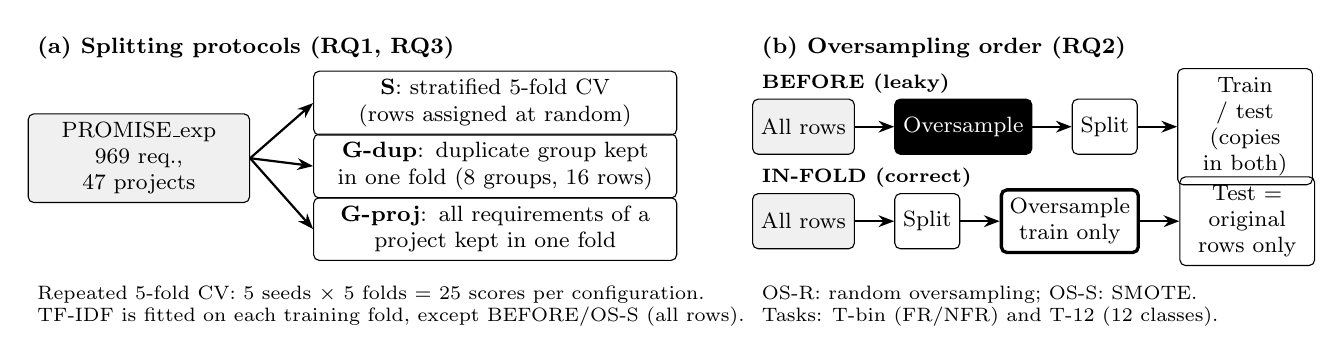
\begin{tikzpicture}[
  font=\footnotesize,
  box/.style={draw, rounded corners=2pt, align=center, minimum height=7mm, inner sep=3pt},
  data/.style={box, fill=gray!12},
  bad/.style={box, fill=black, text=white},
  good/.style={box, fill=white, very thick},
  arr/.style={-{Stealth[length=2mm]}, thick},
  lbl/.style={font=\footnotesize\bfseries, anchor=west}
]
% ---------- (a) splitting protocols ----------
\node[lbl] at (0,0) {(a) Splitting protocols (RQ1, RQ3)};
\node[data, anchor=west, text width=2.6cm] (d) at (0,-1.4) {PROMISE\_exp\\969 req., 47 projects};
\node[box, right=8mm of d, yshift=7mm, text width=4.4cm] (s) {\textbf{S}: stratified 5-fold CV\\(rows assigned at random)};
\node[box, right=8mm of d, yshift=-1mm, text width=4.4cm] (gd) {\textbf{G-dup}: duplicate group kept\\in one fold (8 groups, 16 rows)};
\node[box, right=8mm of d, yshift=-9mm, text width=4.4cm] (gp) {\textbf{G-proj}: all requirements of a\\project kept in one fold};
\draw[arr] (d.east) -- (s.west);
\draw[arr] (d.east) -- (gd.west);
\draw[arr] (d.east) -- (gp.west);
\node[font=\scriptsize, align=left, anchor=north west] at (0,-2.9) {Repeated 5-fold CV: 5 seeds $\times$ 5 folds = 25 scores per configuration.\\TF-IDF is fitted on each training fold, except BEFORE/OS-S (all rows).};

% ---------- (b) oversampling order ----------
\begin{scope}[xshift=9.2cm]
\node[lbl] at (0,0) {(b) Oversampling order (RQ2)};
\node[font=\scriptsize\bfseries, anchor=west] at (0,-0.45) {BEFORE (leaky)};
\node[data, anchor=west] (d2) at (0,-1.0) {All rows};
\node[bad, right=5mm of d2] (os1) {Oversample};
\node[box, right=5mm of os1] (sp1) {Split};
\node[box, right=5mm of sp1, text width=1.5cm] (t1) {Train / test\\(copies in both)};
\draw[arr] (d2) -- (os1); \draw[arr] (os1) -- (sp1); \draw[arr] (sp1) -- (t1);

\node[font=\scriptsize\bfseries, anchor=west] at (0,-1.65) {IN-FOLD (correct)};
\node[data, anchor=west] (d3) at (0,-2.2) {All rows};
\node[box, right=5mm of d3] (sp2) {Split};
\node[good, right=5mm of sp2] (os2) {Oversample\\train only};
\node[box, right=5mm of os2, text width=1.5cm] (t2) {Test = original\\rows only};
\draw[arr] (d3) -- (sp2); \draw[arr] (sp2) -- (os2); \draw[arr] (os2) -- (t2);
\node[font=\scriptsize, align=left, anchor=north west] at (0,-2.9) {OS-R: random oversampling; OS-S: SMOTE.\\ Tasks: T-bin (FR/NFR) and T-12 (12 classes).};
\end{scope}
\end{tikzpicture}
 inside a figure* environment.
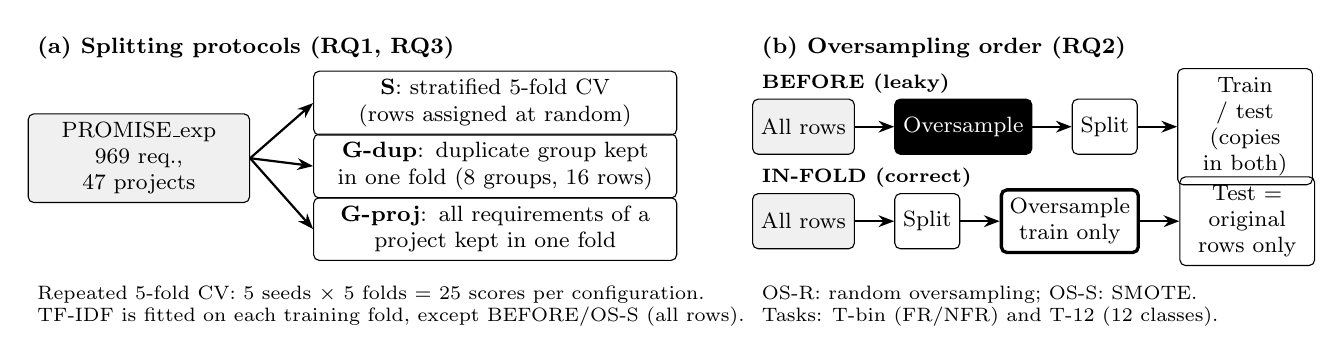
\begin{tikzpicture}[
  font=\footnotesize,
  box/.style={draw, rounded corners=2pt, align=center, minimum height=7mm, inner sep=3pt},
  data/.style={box, fill=gray!12},
  bad/.style={box, fill=black, text=white},
  good/.style={box, fill=white, very thick},
  arr/.style={-{Stealth[length=2mm]}, thick},
  lbl/.style={font=\footnotesize\bfseries, anchor=west}
]
% ---------- (a) splitting protocols ----------
\node[lbl] at (0,0) {(a) Splitting protocols (RQ1, RQ3)};
\node[data, anchor=west, text width=2.6cm] (d) at (0,-1.4) {PROMISE\_exp\\969 req., 47 projects};
\node[box, right=8mm of d, yshift=7mm, text width=4.4cm] (s) {\textbf{S}: stratified 5-fold CV\\(rows assigned at random)};
\node[box, right=8mm of d, yshift=-1mm, text width=4.4cm] (gd) {\textbf{G-dup}: duplicate group kept\\in one fold (8 groups, 16 rows)};
\node[box, right=8mm of d, yshift=-9mm, text width=4.4cm] (gp) {\textbf{G-proj}: all requirements of a\\project kept in one fold};
\draw[arr] (d.east) -- (s.west);
\draw[arr] (d.east) -- (gd.west);
\draw[arr] (d.east) -- (gp.west);
\node[font=\scriptsize, align=left, anchor=north west] at (0,-2.9) {Repeated 5-fold CV: 5 seeds $\times$ 5 folds = 25 scores per configuration.\\TF-IDF is fitted on each training fold, except BEFORE/OS-S (all rows).};

% ---------- (b) oversampling order ----------
\begin{scope}[xshift=9.2cm]
\node[lbl] at (0,0) {(b) Oversampling order (RQ2)};
\node[font=\scriptsize\bfseries, anchor=west] at (0,-0.45) {BEFORE (leaky)};
\node[data, anchor=west] (d2) at (0,-1.0) {All rows};
\node[bad, right=5mm of d2] (os1) {Oversample};
\node[box, right=5mm of os1] (sp1) {Split};
\node[box, right=5mm of sp1, text width=1.5cm] (t1) {Train / test\\(copies in both)};
\draw[arr] (d2) -- (os1); \draw[arr] (os1) -- (sp1); \draw[arr] (sp1) -- (t1);

\node[font=\scriptsize\bfseries, anchor=west] at (0,-1.65) {IN-FOLD (correct)};
\node[data, anchor=west] (d3) at (0,-2.2) {All rows};
\node[box, right=5mm of d3] (sp2) {Split};
\node[good, right=5mm of sp2] (os2) {Oversample\\train only};
\node[box, right=5mm of os2, text width=1.5cm] (t2) {Test = original\\rows only};
\draw[arr] (d3) -- (sp2); \draw[arr] (sp2) -- (os2); \draw[arr] (os2) -- (t2);
\node[font=\scriptsize, align=left, anchor=north west] at (0,-2.9) {OS-R: random oversampling; OS-S: SMOTE.\\ Tasks: T-bin (FR/NFR) and T-12 (12 classes).};
\end{scope}
\end{tikzpicture}
}
\caption{Evaluation design. (a) The three splitting protocols compared in RQ1 (S vs.\ G-dup, S vs.\ G-proj) and used for RQ3. (b) The two oversampling orders compared in RQ2; in BEFORE the test folds can contain copies or synthetic neighbours of training rows.}
\label{fig:design}
\Description{Diagram of the three splitting protocols (stratified, duplicate-grouped, project-grouped) and of oversampling before versus inside the training fold.}
\end{figure*}

We wrote down the data, pipeline, models, protocols, statistical decision rule and wording rules in a protocol and locked it before training any model. This section summarises that protocol.

\subsection{Datasets and tasks}

\textbf{PROMISE\_exp.} Our primary benchmark is PROMISE\_exp~\cite{lima2019}, the expanded version of the PROMISE NFR dataset~\cite{clelandhuang2007}. We used a public mirror and recorded its SHA-256 hash. It has 969 requirements (444 FR, 525 NFR) from 47 projects, with 1 to 92 requirements per project. Each requirement carries one of 12 codes: F (444), SE (125), US (85), O (77), PE (67), LF (49), A (31), MN (24), SC (22), FT (18), L (15) and PO (12). The binary task \emph{T-bin} maps F to FR and every other code to NFR; \emph{T-12} keeps the 12 classes.

\textbf{Duplicate groups.} We found 3 groups of exact duplicates. Character 3- to 5-gram TF-IDF cosine similarity between all requirement pairs flagged 14 near-duplicate candidates (similarity $\geq 0.90$), and manual review confirmed 5 of them. This gives 8 duplicate groups with 16 rows and no label conflicts. Under stratified random CV, 6 to 8 of these groups cross folds; the number depends on the seed.

\textbf{Replication data.} To check whether the RQ2 findings carry over, we repeated the binary analysis on the data released by Dalpiaz et al.~\cite{dalpiaz2019,dalpiaz2019data}: the dronology, leeds, reqview and wasp datasets. We mapped requirements with IsQuality~$=1$ to NFR, including 81 requirements labelled both functional and quality, and requirements with only IsFunctional~$=1$ to FR. Dropping 4 unlabelled rows leaves 327 requirements (187 FR, 140 NFR), with no duplicates and no overlap with PROMISE\_exp. For a sensitivity analysis (``no-both''), we removed the 81 requirements labelled both ways, which leaves 246 rows (187 FR, 59 NFR), and evaluated them under stratified CV only.

\subsection{Pipeline and models}

All models share one pipeline. Preprocessing (P0) applies Unicode NFKC normalisation and lowercasing, expands negative contractions and collapses whitespace; it removes no stop words and does no lemmatisation. Features are TF-IDF word unigrams and bigrams (\texttt{min\_df}~$=2$, sublinear term frequency). The vectoriser is fitted on each training fold, except for BEFORE with OS-S, where it is fitted on all rows before splitting.

We used seven scikit-learn classifiers~\cite{pedregosa2011} with fixed hyperparameters and no tuning. M0 is a most-frequent dummy classifier that sets a floor. M1 is logistic regression ($C=1$), M2 a linear SVM ($C=1$), M3 a random forest with 300 trees and M4 complement naive Bayes ($\alpha=1$). M5 is hard voting over M1, M2 and M3. M6 stacks the same three models with a logistic-regression meta-learner; its meta-features come from an inner 5-fold CV on the outer training rows, with the same splitter type as the outer protocol. A unit test checks that no outer test row enters inner training.

\subsection{Evaluation protocols}

On PROMISE\_exp we compared three 5-fold protocols (Fig.~\ref{fig:design}a). \emph{S} is stratified random CV (\texttt{StratifiedKFold}). \emph{G-dup} uses \texttt{StratifiedGroupKFold} with the duplicate groups, so all copies of a requirement fall into one fold. \emph{G-proj} uses \texttt{StratifiedGroupKFold} with the project ID, so every test fold holds only projects unseen in training. These repeated 5-fold configurations use 5 seeds (42, 123, 2026, 3407 and 9917), giving 25 fold scores per configuration. On the Dalpiaz data, stratified CV (S) is also repeated this way; leave-one-dataset-out (\emph{LODO}) is a single deterministic run with 4 fold scores, one for each held-out dataset. Test folds held 193 or 194 rows under S and G-dup and 172 to 245 rows under G-proj. RQ1 and RQ3 use T-bin without oversampling, and G-dup is the primary protocol for RQ3.

\subsection{Oversampling conditions}

For RQ2 we used two oversamplers from imbalanced-learn~\cite{lemaitre2017}: random oversampling (OS-R) and SMOTE~\cite{chawla2002} on the TF-IDF vectors (OS-S). We compared three conditions (Fig.~\ref{fig:design}b). \emph{NONE} applies no oversampling. \emph{IN-FOLD} oversamples only the training part of each fold, so test folds contain original requirements only. \emph{BEFORE} oversamples the whole dataset and then splits it, as several reviewed studies do; for OS-S this also means fitting TF-IDF on all rows. BEFORE test folds can therefore contain exact copies (OS-R) or synthetic neighbours (OS-S) of training rows. Because BEFORE splits a larger, oversampled set, its test folds are different rows from the IN-FOLD test folds, and we compare the two conditions descriptively. RQ2 uses protocol S, models M1 to M5 and both tasks. The Dalpiaz replication uses T-bin.

\subsection{Metrics and statistical analysis}

The primary metric is macro-F1, computed on each test fold and averaged across folds: 25 scores for repeated 5-fold CV and 4 for LODO. We also recorded accuracy, macro precision and macro recall. How we analyse a comparison depends on whether both sides are evaluated on the same test rows.

\textbf{Comparisons on the same splits (RQ3).} Models under the same protocol share the splits of each seed, so their fold scores are paired. For each comparison of A against B we computed the mean paired difference $\Delta$, its standard deviation and a 95\% confidence interval with the corrected repeated $k$-fold $t$-test~\cite{nadeau2003,bouckaert2004}. The test uses the actual test/training size ratio of the folds. We adjusted $p$-values with the Holm method~\cite{holm1979} within each family: RQ3 under G-dup (8 tests) and under S (8 tests). We call a difference \emph{clear} only if $|\Delta| \geq 0.01$ and the Holm-adjusted $p < 0.05$; otherwise we report \emph{no clear difference}.

\textbf{Comparisons across protocols or oversampling conditions (RQ1, RQ2, replication).} S, G-dup and G-proj produce different test folds. At the same (seed, fold) index, none of the 25 S folds equals the matching G-dup or G-proj fold, and they share only about 20\% of their rows, which is the overlap expected by chance. BEFORE test folds come from the oversampled set and hold 210 to 1066 rows instead of 193 or 194. Pairing such fold scores by index would break the assumption of the paired test. We therefore report the mean and standard deviation of macro-F1 over each side's own 25 folds, and $\Delta$ as the difference of the two means. The protocol had planned paired tests for these families; after the runs we replaced them with descriptive reporting in a documented amendment, without re-running any model. Kendall's $\tau$ measures agreement between model rankings. S vs.\ LODO (25 vs.\ 4 folds), NONE vs.\ IN-FOLD and the no-both analysis are descriptive as well.

\begin{table*}[t]
\centering
\caption{RQ1: macro-F1 under stratified CV (S), duplicate-grouped CV (G-dup) and project-grouped CV (G-proj) on PROMISE\_exp, T-bin, no oversampling. $\Delta$ = S $-$ grouped (difference of means). Descriptive only: the protocols use different test folds, so no paired test is applied (mean $\pm$ SD over 5 seeds $\times$ 5 folds).}
\label{tab:rq1}
\small
\setlength{\tabcolsep}{4pt}
\begin{tabular}{lrrrrr}
\toprule
& \multicolumn{3}{c}{Macro-F1} & \multicolumn{2}{c}{$\Delta$} \\
\cmidrule(lr){2-4}\cmidrule(lr){5-6}
Model & S & G-dup & G-proj & S $-$ G-dup & S $-$ G-proj \\
\midrule
M0 & $0.351 \pm 0.000$ & $0.351 \pm 0.000$ & $0.352 \pm 0.008$ & -- & -- \\
M1 & $0.876 \pm 0.020$ & $0.878 \pm 0.025$ & $0.694 \pm 0.094$ & $-0.002$ & $+0.182$ \\
M2 & $0.893 \pm 0.019$ & $0.891 \pm 0.018$ & $0.722 \pm 0.061$ & $+0.001$ & $+0.171$ \\
M3 & $0.851 \pm 0.031$ & $0.853 \pm 0.022$ & $0.661 \pm 0.113$ & $-0.001$ & $+0.190$ \\
M4 & $0.889 \pm 0.019$ & $0.884 \pm 0.025$ & $0.755 \pm 0.055$ & $+0.005$ & $+0.134$ \\
M5 & $0.882 \pm 0.023$ & $0.885 \pm 0.019$ & $0.705 \pm 0.083$ & $-0.003$ & $+0.176$ \\
M6 & $0.891 \pm 0.018$ & $0.894 \pm 0.019$ & $0.749 \pm 0.052$ & $-0.003$ & $+0.142$ \\
\bottomrule
\end{tabular}
\end{table*}

\begin{table*}[t]
\centering
\caption{RQ2: macro-F1 when oversampling is applied to the whole dataset before splitting (BEFORE) versus inside each training fold only (IN-FOLD), PROMISE\_exp, stratified CV. OS-R: random oversampling; OS-S: SMOTE. $\Delta$ = BEFORE $-$ IN-FOLD (difference of means). Descriptive only: BEFORE test folds are drawn from the oversampled set, so they are not the IN-FOLD test rows and no paired test is applied (mean $\pm$ SD over 5 seeds $\times$ 5 folds).}
\label{tab:rq2}
\small
\setlength{\tabcolsep}{4pt}
\begin{tabular}{llrrrrrr}
\toprule
& & \multicolumn{3}{c}{T-bin (FR vs NFR)} & \multicolumn{3}{c}{T-12 (12 classes)} \\
\cmidrule(lr){3-5}\cmidrule(lr){6-8}
Model & OS & BEFORE & IN-FOLD & $\Delta$ & BEFORE & IN-FOLD & $\Delta$ \\
\midrule
M1 & OS-R & $0.899 \pm 0.021$ & $0.878 \pm 0.019$ & $+0.020$ & $0.989 \pm 0.003$ & $0.597 \pm 0.064$ & $+0.392$ \\
M1 & OS-S & $0.900 \pm 0.025$ & $0.879 \pm 0.022$ & $+0.021$ & $0.988 \pm 0.003$ & $0.589 \pm 0.063$ & $+0.399$ \\
M2 & OS-R & $0.917 \pm 0.017$ & $0.893 \pm 0.020$ & $+0.024$ & $0.992 \pm 0.003$ & $0.593 \pm 0.075$ & $+0.399$ \\
M2 & OS-S & $0.920 \pm 0.015$ & $0.894 \pm 0.018$ & $+0.026$ & $0.992 \pm 0.003$ & $0.595 \pm 0.070$ & $+0.398$ \\
M3 & OS-R & $0.882 \pm 0.021$ & $0.855 \pm 0.027$ & $+0.027$ & $0.994 \pm 0.003$ & $0.506 \pm 0.061$ & $+0.488$ \\
M3 & OS-S & $0.878 \pm 0.023$ & $0.855 \pm 0.032$ & $+0.023$ & $0.986 \pm 0.003$ & $0.495 \pm 0.058$ & $+0.491$ \\
M4 & OS-R & $0.903 \pm 0.021$ & $0.888 \pm 0.018$ & $+0.015$ & $0.967 \pm 0.006$ & $0.526 \pm 0.040$ & $+0.441$ \\
M4 & OS-S & $0.905 \pm 0.019$ & $0.890 \pm 0.018$ & $+0.015$ & $0.951 \pm 0.006$ & $0.525 \pm 0.049$ & $+0.425$ \\
M5 & OS-R & $0.909 \pm 0.023$ & $0.886 \pm 0.022$ & $+0.023$ & $0.992 \pm 0.003$ & $0.595 \pm 0.070$ & $+0.398$ \\
M5 & OS-S & $0.908 \pm 0.022$ & $0.885 \pm 0.023$ & $+0.023$ & $0.993 \pm 0.002$ & $0.587 \pm 0.065$ & $+0.406$ \\
\bottomrule
\end{tabular}
\end{table*}


\subsection{Reproducibility}

We locked the protocol on 16 October 2026, before running any model, and re-ran no configuration to change a result. The runs comprised 21 configurations for RQ1 (525 fold fits), 50 for RQ2 (1250) and 35 for the Dalpiaz replication (770). Each run logged the git commit, dataset hashes, seeds and package versions. A complete re-run on 18 October 2026 reproduced every per-fold score bit for bit: the SHA-256 hashes of all fold-score files were identical. Code, split indices, per-fold scores and analysis scripts are public (Section~\ref{sec:conclusion}).

\section{Results}
\label{sec:results}

\begin{figure}[t]
\centering
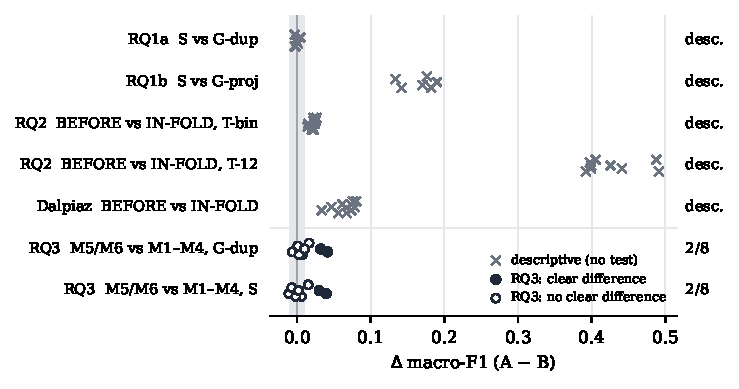
\includegraphics[width=\columnwidth]{figures/summary_deltas.pdf}
\caption{Mean difference in macro-F1 for every planned comparison (one marker per model or model$\times$oversampler). Crosses: comparisons across protocols or oversampling conditions, reported descriptively (difference of means; different test folds). Circles: RQ3, tested on the same splits; filled = clear difference ($|\Delta| \geq 0.01$ and Holm-adjusted $p < 0.05$), hollow = no clear difference. Grey band: $|\Delta| < 0.01$. Right: clear differences per tested family.}
\label{fig:summary}
\Description{Dot plot of mean macro-F1 differences for every planned comparison, grouped by research question, with a grey band marking differences below 0.01.}
\end{figure}

Fig.~\ref{fig:summary} shows all planned comparisons. For RQ1, RQ2 and the replication the test folds differ, so these comparisons are differences of means (Section~\ref{sec:method}). Two of them are large compared with the variation between folds: S vs.\ G-proj and BEFORE vs.\ IN-FOLD on the 12-class task. In RQ3, where models share the same splits, 2 of 8 comparisons show a clear difference under G-dup and under S. The dummy classifier M0 scored a macro-F1 of about 0.35 under every protocol.

\subsection{RQ1: Duplicate- and project-grouped evaluation}
\begin{table*}[t]
\centering
\caption{RQ1: macro-F1 under stratified CV (S), duplicate-grouped CV (G-dup) and project-grouped CV (G-proj) on PROMISE\_exp, T-bin, no oversampling. $\Delta$ = S $-$ grouped (difference of means). Descriptive only: the protocols use different test folds, so no paired test is applied (mean $\pm$ SD over 5 seeds $\times$ 5 folds).}
\label{tab:rq1}
\small
\setlength{\tabcolsep}{4pt}
\begin{tabular}{lrrrrr}
\toprule
& \multicolumn{3}{c}{Macro-F1} & \multicolumn{2}{c}{$\Delta$} \\
\cmidrule(lr){2-4}\cmidrule(lr){5-6}
Model & S & G-dup & G-proj & S $-$ G-dup & S $-$ G-proj \\
\midrule
M0 & $0.351 \pm 0.000$ & $0.351 \pm 0.000$ & $0.352 \pm 0.008$ & -- & -- \\
M1 & $0.876 \pm 0.020$ & $0.878 \pm 0.025$ & $0.694 \pm 0.094$ & $-0.002$ & $+0.182$ \\
M2 & $0.893 \pm 0.019$ & $0.891 \pm 0.018$ & $0.722 \pm 0.061$ & $+0.001$ & $+0.171$ \\
M3 & $0.851 \pm 0.031$ & $0.853 \pm 0.022$ & $0.661 \pm 0.113$ & $-0.001$ & $+0.190$ \\
M4 & $0.889 \pm 0.019$ & $0.884 \pm 0.025$ & $0.755 \pm 0.055$ & $+0.005$ & $+0.134$ \\
M5 & $0.882 \pm 0.023$ & $0.885 \pm 0.019$ & $0.705 \pm 0.083$ & $-0.003$ & $+0.176$ \\
M6 & $0.891 \pm 0.018$ & $0.894 \pm 0.019$ & $0.749 \pm 0.052$ & $-0.003$ & $+0.142$ \\
\bottomrule
\end{tabular}
\end{table*}


\textbf{S vs.\ G-dup.} Grouping duplicates left the estimates almost unchanged (Table~\ref{tab:rq1}). $\Delta$ ranged from $-0.003$ to $+0.005$. That is below the 0.01 threshold for every model and far below the fold standard deviation (0.018 to 0.031 under S, 0.018 to 0.025 under G-dup). Kendall's $\tau$ between the two rankings is 0.733 (Table~\ref{tab:kendall}). PROMISE\_exp has only 8 duplicate groups (16 of 969 rows), so this negative result holds for this dataset and does not show that duplicates never matter.

\textbf{S vs.\ G-proj.} Keeping each project in one fold lowered macro-F1 for all six models, from 0.851 to 0.893 under S to 0.661 to 0.755 under G-proj. The drop ranged from 0.134 (M4) to 0.190 (M3). Scores also varied more between folds, with a standard deviation of 0.052 to 0.113 under G-proj against 0.018 to 0.031 under S. The ranking changed (Kendall's $\tau = 0.600$): M2 was best under S (0.893) and M4 under G-proj (0.755).

\textbf{Answer to RQ1:} \emph{Grouping duplicates changes macro-F1 on PROMISE\_exp by less than 0.01 for every model. Testing on unseen projects lowers macro-F1 by 0.134 to 0.190 for every model and changes the model ranking.}

\subsection{RQ2: Oversampling before vs.\ inside the training fold}
\begin{table*}[t]
\centering
\caption{RQ2: macro-F1 when oversampling is applied to the whole dataset before splitting (BEFORE) versus inside each training fold only (IN-FOLD), PROMISE\_exp, stratified CV. OS-R: random oversampling; OS-S: SMOTE. $\Delta$ = BEFORE $-$ IN-FOLD (difference of means). Descriptive only: BEFORE test folds are drawn from the oversampled set, so they are not the IN-FOLD test rows and no paired test is applied (mean $\pm$ SD over 5 seeds $\times$ 5 folds).}
\label{tab:rq2}
\small
\setlength{\tabcolsep}{4pt}
\begin{tabular}{llrrrrrr}
\toprule
& & \multicolumn{3}{c}{T-bin (FR vs NFR)} & \multicolumn{3}{c}{T-12 (12 classes)} \\
\cmidrule(lr){3-5}\cmidrule(lr){6-8}
Model & OS & BEFORE & IN-FOLD & $\Delta$ & BEFORE & IN-FOLD & $\Delta$ \\
\midrule
M1 & OS-R & $0.899 \pm 0.021$ & $0.878 \pm 0.019$ & $+0.020$ & $0.989 \pm 0.003$ & $0.597 \pm 0.064$ & $+0.392$ \\
M1 & OS-S & $0.900 \pm 0.025$ & $0.879 \pm 0.022$ & $+0.021$ & $0.988 \pm 0.003$ & $0.589 \pm 0.063$ & $+0.399$ \\
M2 & OS-R & $0.917 \pm 0.017$ & $0.893 \pm 0.020$ & $+0.024$ & $0.992 \pm 0.003$ & $0.593 \pm 0.075$ & $+0.399$ \\
M2 & OS-S & $0.920 \pm 0.015$ & $0.894 \pm 0.018$ & $+0.026$ & $0.992 \pm 0.003$ & $0.595 \pm 0.070$ & $+0.398$ \\
M3 & OS-R & $0.882 \pm 0.021$ & $0.855 \pm 0.027$ & $+0.027$ & $0.994 \pm 0.003$ & $0.506 \pm 0.061$ & $+0.488$ \\
M3 & OS-S & $0.878 \pm 0.023$ & $0.855 \pm 0.032$ & $+0.023$ & $0.986 \pm 0.003$ & $0.495 \pm 0.058$ & $+0.491$ \\
M4 & OS-R & $0.903 \pm 0.021$ & $0.888 \pm 0.018$ & $+0.015$ & $0.967 \pm 0.006$ & $0.526 \pm 0.040$ & $+0.441$ \\
M4 & OS-S & $0.905 \pm 0.019$ & $0.890 \pm 0.018$ & $+0.015$ & $0.951 \pm 0.006$ & $0.525 \pm 0.049$ & $+0.425$ \\
M5 & OS-R & $0.909 \pm 0.023$ & $0.886 \pm 0.022$ & $+0.023$ & $0.992 \pm 0.003$ & $0.595 \pm 0.070$ & $+0.398$ \\
M5 & OS-S & $0.908 \pm 0.022$ & $0.885 \pm 0.023$ & $+0.023$ & $0.993 \pm 0.002$ & $0.587 \pm 0.065$ & $+0.406$ \\
\bottomrule
\end{tabular}
\end{table*}


\textbf{T-bin.} On the binary task, BEFORE gave higher estimates than IN-FOLD for every model and oversampler (Table~\ref{tab:rq2}): 0.878 to 0.920 against 0.855 to 0.894, a difference of $+0.015$ to $+0.027$. The direction is consistent, but the size is of the same order as the fold standard deviation (0.015 to 0.032).

\textbf{T-12.} On the 12-class task, BEFORE reached 0.951 to 0.994 and IN-FOLD 0.495 to 0.597, a difference of $+0.392$ to $+0.491$ for all ten model and oversampler combinations. The fold standard deviation was 0.002 to 0.006 under BEFORE and 0.040 to 0.075 under IN-FOLD, many times smaller than the difference. M3 showed the largest gaps ($+0.488$ with OS-R, $+0.491$ with OS-S).

\textbf{NONE vs.\ IN-FOLD.} Table~\ref{tab:none_infold} (descriptive) separates the effect of oversampling itself. On T-12, in-fold oversampling raised macro-F1 for M1 ($+0.30$), M5 ($+0.17$ to $+0.18$) and M3 ($+0.11$ to $+0.12$), barely changed M2 ($+0.03$) and lowered M4 ($-0.04$). Without leakage, the 12-class task scores 0.292 to 0.563 (NONE) or 0.495 to 0.597 (IN-FOLD), far below the 0.951 to 0.994 obtained with BEFORE. On T-bin, IN-FOLD and NONE differ by only $-0.001$ to $+0.004$.

\textbf{Answer to RQ2:} \emph{Oversampling before splitting raises macro-F1 on the 12-class task by 0.392 to 0.491 for all models and both oversamplers. A task that reaches at most 0.597 then appears to score 0.951 to 0.994. On the binary task the increase is 0.015 to 0.027, of the same order as the variation between folds.}

\subsection{RQ3: Ensembles under leakage-aware evaluation}
\begin{table}[t]
\centering
\caption{RQ3: ensembles (M5 hard voting, M6 stacking) versus single classifiers M1--M4, PROMISE\_exp, T-bin, macro-F1. $\Delta$ = ensemble $-$ single; 95\% CI from the corrected $t$-test (unadjusted). G-dup is the primary protocol; S is reported for comparison. Bold $\Delta$: clear difference ($|\Delta| \geq 0.01$ and Holm-adjusted $p < 0.05$, corrected repeated $k$-fold $t$-test).}
\label{tab:rq3}
\footnotesize
\setlength{\tabcolsep}{3pt}
\begin{tabular}{lrrrrr}
\toprule
& \multicolumn{3}{c}{G-dup (primary)} & \multicolumn{2}{c}{S} \\
\cmidrule(lr){2-4}\cmidrule(lr){5-6}
Comparison & $\Delta$ & 95\% CI & $p_{\mathrm{Holm}}$ & $\Delta$ & $p_{\mathrm{Holm}}$ \\
\midrule
M5 vs M1 & $+0.007$ & $[-0.002, +0.017]$ & $0.707$ & $+0.006$ & $1.000$ \\
M5 vs M2 & $-0.006$ & $[-0.022, +0.009]$ & $1.000$ & $-0.011$ & $0.280$ \\
M5 vs M3 & $\mathbf{+0.032}$ & $[+0.016, +0.048]$ & $0.003$ & $\mathbf{+0.030}$ & $0.013$ \\
M5 vs M4 & $+0.001$ & $[-0.014, +0.016]$ & $1.000$ & $-0.007$ & $1.000$ \\
M6 vs M1 & $+0.017$ & $[-0.004, +0.038]$ & $0.707$ & $+0.015$ & $0.280$ \\
M6 vs M2 & $+0.003$ & $[-0.007, +0.012]$ & $1.000$ & $-0.002$ & $1.000$ \\
M6 vs M3 & $\mathbf{+0.042}$ & $[+0.024, +0.059]$ & $<0.001$ & $\mathbf{+0.040}$ & $0.007$ \\
M6 vs M4 & $+0.010$ & $[-0.007, +0.028]$ & $0.916$ & $+0.002$ & $1.000$ \\
\bottomrule
\end{tabular}
\end{table}


Under G-dup, both ensembles were clearly better than the random forest and no other model (Table~\ref{tab:rq3}): M5 vs.\ M3 $\Delta = +0.032$ (Holm-adjusted $p = 0.003$) and M6 vs.\ M3 $\Delta = +0.042$ ($p < 0.001$). The other 6 comparisons, against M1, M2 and M4, show no clear difference; their $\Delta$ ranges from $-0.006$ to $+0.017$ and all their confidence intervals include zero. Under S the pattern repeats (2/8), with M5 vs.\ M3 at $+0.030$ and M6 vs.\ M3 at $+0.040$.

\textbf{Answer to RQ3:} \emph{Under G-dup, hard voting and stacking are clearly better only than the random forest (M5 $+0.032$, M6 $+0.042$). Against logistic regression, the linear SVM and complement naive Bayes there is no clear difference.}

\subsection{Replication on the Dalpiaz et al.\ dataset}
\begin{table}[t]
\centering
\caption{Replication on the Dalpiaz et al.\ dataset ($n=327$, four datasets), T-bin, macro-F1 (means). Left: stratified CV (S) vs leave-one-dataset-out (LODO). Right: $\Delta$ = BEFORE $-$ IN-FOLD. All comparisons are descriptive (different test folds; S has 25 folds, LODO 4).}
\label{tab:dalpiaz}
\small
\setlength{\tabcolsep}{4pt}
\begin{tabular}{lrrrrr}
\toprule
& \multicolumn{3}{c}{Evaluation protocol} & \multicolumn{2}{c}{BEFORE $-$ IN-FOLD} \\
\cmidrule(lr){2-4}\cmidrule(lr){5-6}
Model & S & LODO & $\Delta$ & OS-R & OS-S \\
\midrule
M1 & $0.709$ & $0.466$ & $+0.244$ & $+0.056$ & $+0.074$ \\
M2 & $0.746$ & $0.491$ & $+0.256$ & $+0.047$ & $+0.073$ \\
M3 & $0.713$ & $0.405$ & $+0.308$ & $+0.081$ & $+0.067$ \\
M4 & $0.726$ & $0.511$ & $+0.214$ & $+0.034$ & $+0.079$ \\
M5 & $0.731$ & $0.493$ & $+0.238$ & $+0.062$ & $+0.076$ \\
\bottomrule
\end{tabular}
\end{table}


On the Dalpiaz data (T-bin), BEFORE again beat IN-FOLD for every model and oversampler, by $+0.034$ to $+0.081$ (BEFORE 0.775 to 0.822, IN-FOLD 0.716 to 0.754; Table~\ref{tab:dalpiaz}). As on PROMISE\_exp T-bin, these differences have a consistent direction and a size comparable to the fold standard deviation (0.039 to 0.066). Testing on an unseen dataset (LODO) gave 0.405 to 0.511, against 0.709 to 0.746 under S, a drop of 0.21 to 0.31. Kendall's $\tau$ between the S and LODO rankings is 0.20. Removing the 81 requirements labelled both functional and quality (Table~\ref{tab:noboth}) raised M2 to M5 by $+0.035$ to $+0.074$ and lowered M1 by 0.103.

\subsection{Error analysis}

We inspected 30 misclassified requirements from PROMISE\_exp (T-bin, G-dup, seed 42): 15 errors of the linear SVM (M2) and 15 of hard voting (M5), each with eight true-NFR and seven true-FR rows. We did not change any ground-truth label.

Both authors assigned an error category to each row and then reconciled their disagreements. Their initial categories agreed on 15 of 30 rows (Cohen's $\kappa = 0.391$). Both used AI assistance while labelling, so this figure is not an agreement between fully independent, unaided raters.

After reconciliation, the most frequent category was \emph{ambiguous or underspecified} (8 rows), for example a requirement to use stored e-mail addresses as the primary means of communication. \emph{Mixed FR/NFR} followed with 7 rows, such as a list of dispute cases that ``must be color coded for easy identification''. Six rows were a \emph{functional verb in an NFR}: the security requirement ``The system shall utilize HTTPS communication to ensure data confidentiality'' was predicted as FR. The remaining rows were a \emph{quality keyword in an FR} (4), for example an alert after a failed login, a \emph{possible annotation issue} (2), \emph{other} (2) and \emph{short or low context} (1). Rows P0809 and P0752 contain the same sentence apart from punctuation; they form one duplicate group, and G-dup puts them in the same fold.

The three largest categories cover 21 of the 30 errors. The moderate initial agreement suggests that many errors have no single obvious cause. These categories are qualitative judgements about 30 selected errors, not verified explanations of model behaviour, and their proportions do not generalise to the full dataset.

\section{Discussion}
\label{sec:discussion}

\textbf{Why BEFORE inflates T-12 so much and T-bin so little.} When the whole dataset is oversampled before splitting, test folds can contain exact copies (OS-R) or synthetic neighbours (OS-S) related to training rows. T-12 has rare classes such as PO (12 rows) and L (15 rows), which are oversampled many times to approach the 444 F rows. This creates substantial opportunity for overlap between training and test data; we did not directly measure the share of rare-class test rows with an exact training copy. Macro-F1 weighs each class equally and rises to between 0.951 and 0.994. On T-bin the two classes are close in size (444 vs.\ 525), fewer rows need to be added, and the increase stays at 0.015 to 0.027. BEFORE on T-12 yields values in the same range as the 98\% to 99\% reported by studies that appear to oversample before splitting~\cite{metu2024hybrid,baskoro2021systematic}. Our data cannot show that those results are wrong, because data versions, splits and metrics differ. They show that the BEFORE practice alone produces such numbers on a task whose macro-F1 without leakage is at most 0.597 in our setup.

\textbf{Duplicates: a negative finding on this dataset.} Grouping duplicates changed macro-F1 on PROMISE\_exp by less than 0.01, because only 8 groups (16 rows) exist. Duplicates may still matter elsewhere. In source code, duplication inflated results considerably~\cite{allamanis2019adverse}, and larger, scraped or merged requirement corpora may contain far more duplicates.

\textbf{Random CV vs.\ unseen projects.} Under G-proj, macro-F1 dropped by 0.134 to 0.190, fold scores varied more and the model ranking changed. We do not read this drop as leakage. Random CV estimates performance on new requirements from projects already seen in training, while a practitioner usually applies a classifier to a new project with its own vocabulary and class balance. Here the model chosen by random CV (M2) is not the one that generalises best to unseen projects (M4). The Dalpiaz LODO results, with a drop of 0.21 to 0.31, point the same way.

\textbf{Ensembles.} Hard voting and stacking beat only the random forest; against the linear models and complement naive Bayes there was no clear difference. M1 and M2 are both linear models on the same TF-IDF features, so their errors are probably correlated, and combining them adds little. Four of the six reviewed ensemble studies claim improvements without a statistical test (Section~\ref{sec:related}). With a corrected test and Holm adjustment, we find no gain over the best single linear model.

\textbf{Recommendations.} From these results, we recommend that FR/NFR classification studies:
\begin{enumerate}
\item oversample, and fit any vectoriser, inside the training fold only, never before splitting;
\item report how duplicates were handled, group them when splitting, and report the number of duplicate groups;
\item report a project-level or dataset-level evaluation alongside random CV when claiming generalisation;
\item report macro-F1 per fold with repeated CV, and use a corrected paired test with multiple-comparison control before claiming that one model, such as an ensemble, is better; apply paired tests only when both sides use the same test folds;
\item publish code, splits and per-fold scores.
\end{enumerate}

\section{Threats to validity}
\label{sec:threats}

\textbf{Construct validity.} The binary FR/NFR label hides requirements that are both functional and quality-related. The error analysis (7 mixed FR/NFR rows) and the no-both analysis (Table~\ref{tab:noboth}) show that such requirements affect the results. Dalpiaz et al.~\cite{dalpiaz2019} questioned the label quality of PROMISE; we never changed a ground-truth label. The duplicate groups depend on the 0.90 similarity threshold, and one person reviewed the 14 candidate pairs. BEFORE is a simplified version of the practice in the reviewed studies and does not reproduce any paper's exact pipeline, so we present it as a measurement of the practice.

\textbf{Internal validity.} BEFORE splits an oversampled set, so its test folds differ from the IN-FOLD test folds, and the differences mix the effect of leakage with that of a different test distribution. Grouped folds are uneven (172 to 245 rows under G-proj). We fixed the hyperparameters by design. Tuning could change absolute scores and individual model comparisons, but it cannot remove the copies that cause the BEFORE inflation. To limit analyst bias, we locked the protocol, the decision rule and the wording rules before any run and re-ran no configuration. We made one amendment after the runs: on finding that the planned paired tests for RQ1 and RQ2 compared different test folds, we replaced them with descriptive reporting. The amendment removes inferential claims and adds none; the amendment log records it.

\textbf{External validity.} The study uses one main benchmark, PROMISE\_exp, and one small replication on the Dalpiaz et al.\ data. Larger or automatically collected corpora may contain many more duplicates, so the negative RQ1(a) result may not transfer. We evaluated classical models only and did not test transformer or LLM classifiers. The literature review covers only open-access papers whose PDF could be downloaded automatically, so the gap counts may not represent the whole field.

\textbf{Conclusion validity.} Folds of repeated CV are not independent. For RQ3, the corrected repeated $k$-fold $t$-test~\cite{nadeau2003,bouckaert2004} reduces the resulting optimism without removing it, and Holm adjustment~\cite{holm1979} controls the family-wise error rate within each family. RQ1, RQ2 and the replication have no significance test. Their conclusions rest on the size and consistency of the differences relative to the variation between folds: clear-cut for G-proj and T-12, weak for the small T-bin differences. The error analysis covers 30 rows and supports qualitative observations only. Both authors used AI assistance while labelling, so the agreement of 15 of 30 rows ($\kappa = 0.391$) does not come from fully independent raters. A complete re-run reproduced every fold score bit for bit.

\section{Conclusion}
\label{sec:conclusion}
We re-evaluated FR/NFR requirements classifiers on PROMISE\_exp under a protocol locked before any run. Oversampling the whole dataset before splitting raised macro-F1 on the 12-class task by 0.392 to 0.491. A task with a macro-F1 of at most 0.597 without leakage then appears to score 0.951 to 0.994. On the binary task the increase was 0.015 to 0.027. Testing on unseen projects lowered macro-F1 by 0.134 to 0.190 and changed the model ranking, while grouping the 8 duplicate groups in PROMISE\_exp changed macro-F1 by less than 0.01. The ensembles were clearly better than the random forest and no other model.

On T-bin under stratified CV, models M1 to M6 differ by at most 0.042 (0.851 to 0.893), whereas the choice of protocol moved macro-F1 by up to 0.190 and the order of oversampling by up to 0.491 on T-12. Results obtained with oversampling before splitting, or with random CV only, should not be compared with results from leakage-aware or project-level evaluation. A claim that one model is better needs a corrected paired test on the same test folds.

Future work can apply the same protocol to transformer and LLM classifiers and to datasets with more duplicates, and can use the 30 analysed errors as a starting point for a label review.

\section*{Data and code availability}
Code, split indices, per-fold scores and the analysis scripts are available at \url{https://github.com/TaiNguyen66/fr_nfr_ensemble_research}. The PROMISE\_exp file is not redistributed because its license is unknown; the Dalpiaz et al.\ data are available from Zenodo~\cite{dalpiaz2019data}.


\begin{acks}
We thank Mr. Ton That Hoang Minh, FPT University, for supervising this study and for feedback on the evaluation design and the manuscript. The authors used an AI assistant (Claude, Anthropic) to help edit the manuscript text and the analysis scripts. The authors checked all statements, numbers and references against the study data and take full responsibility for the content.
\end{acks}


\appendix
\section{Supplementary results}
Tables~\ref{tab:none_infold}, \ref{tab:kendall} and \ref{tab:noboth} give the descriptive results referred to in Section~\ref{sec:results}.
\begin{table}[H]
\centering
\caption{Effect of correct (IN-FOLD) oversampling against no oversampling (NONE), PROMISE\_exp, stratified CV, macro-F1. OS-R: random oversampling; OS-S: SMOTE. $\Delta$ = IN-FOLD $-$ NONE. Descriptive only.}
\label{tab:none_infold}
\small
\setlength{\tabcolsep}{4pt}
\begin{tabular}{lrrrrr}
\toprule
& & \multicolumn{2}{c}{IN-FOLD, OS-R} & \multicolumn{2}{c}{IN-FOLD, OS-S} \\
\cmidrule(lr){3-4}\cmidrule(lr){5-6}
Model & NONE & F1 & $\Delta$ & F1 & $\Delta$ \\
\midrule
\multicolumn{6}{l}{\textit{T-bin (FR vs NFR)}} \\
M1 & $0.876$ & $0.878$ & $+0.003$ & $0.879$ & $+0.003$ \\
M2 & $0.893$ & $0.893$ & $+0.000$ & $0.894$ & $+0.001$ \\
M3 & $0.851$ & $0.855$ & $+0.004$ & $0.855$ & $+0.004$ \\
M4 & $0.889$ & $0.888$ & $-0.001$ & $0.890$ & $+0.001$ \\
M5 & $0.882$ & $0.886$ & $+0.004$ & $0.885$ & $+0.003$ \\
\midrule
\multicolumn{6}{l}{\textit{T-12 (12 classes)}} \\
M1 & $0.292$ & $0.597$ & $+0.304$ & $0.589$ & $+0.297$ \\
M2 & $0.562$ & $0.593$ & $+0.030$ & $0.595$ & $+0.032$ \\
M3 & $0.386$ & $0.506$ & $+0.120$ & $0.495$ & $+0.109$ \\
M4 & $0.563$ & $0.526$ & $-0.037$ & $0.525$ & $-0.038$ \\
M5 & $0.414$ & $0.595$ & $+0.180$ & $0.587$ & $+0.173$ \\
\bottomrule
\end{tabular}
\end{table}

\begin{table}[H]
\centering
\caption{Agreement of model rankings (mean macro-F1, T-bin, no oversampling) between evaluation protocols (Kendall's $\tau$).}
\label{tab:kendall}
\small
\setlength{\tabcolsep}{4pt}
\begin{tabular}{llp{2.6cm}r}
\toprule
Dataset & Protocols & Models & $\tau$ \\
\midrule
PROMISE\_exp & S vs G-dup & M1, M2, M3, M4, M5, M6 & $0.733$ \\
PROMISE\_exp & S vs G-proj & M1, M2, M3, M4, M5, M6 & $0.600$ \\
Dalpiaz & S vs LODO & M1, M2, M3, M4, M5 & $0.200$ \\
\bottomrule
\end{tabular}
\end{table}

\begin{table}[H]
\centering
\caption{Sensitivity of the Dalpiaz replication to removing requirements labelled both F and Q (T-bin, S, no oversampling; macro-F1 mean $\pm$ SD over 25 folds; full $n=327$, no-both $n=246$). Descriptive only.}
\label{tab:noboth}
\small
\setlength{\tabcolsep}{4pt}
\begin{tabular}{lrrr}
\toprule
Model & Full & No-both & $\Delta$ \\
\midrule
M1 & $0.709 \pm 0.039$ & $0.606 \pm 0.094$ & $-0.103$ \\
M2 & $0.746 \pm 0.043$ & $0.820 \pm 0.040$ & $+0.074$ \\
M3 & $0.713 \pm 0.038$ & $0.775 \pm 0.075$ & $+0.062$ \\
M4 & $0.726 \pm 0.043$ & $0.798 \pm 0.067$ & $+0.072$ \\
M5 & $0.731 \pm 0.038$ & $0.766 \pm 0.067$ & $+0.035$ \\
\bottomrule
\end{tabular}
\end{table}


\bibliographystyle{ACM-Reference-Format}
\bibliography{references}

\end{document}
